\section{Задача 1.24}
\subsection{Задание:}
Решить
$
	\left|
		\begin{matrix}
			2 & x & 6 \\
			3 & 3 & 9 \\
			7 & 4 & 11
		\end{matrix}
	\right|
	= 0
$
\subsection{Решение:}
$
	3 \cdot 11 \cdot x + 2 \cdot 4 \cdot 9 + 2 \cdot 3 \cdot 11 -
	6 \cdot 3 \cdot 4 - 6 \cdot 3 \cdot 7 - 7 \cdot 9 \cdot x = 0
	\\[1ex]
	-30x - 60 = 0
	\\[1ex]
	x = -\dfrac{60}{30} = 2
$
\subsection{Проверим результат в среде Wolfram Mathematica:}
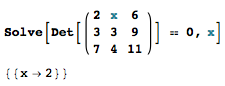
\includegraphics[scale=0.6]{task/1_24/screen.png}
\subsection{Ответ:}
Компьютерная проверка подтвердила полученный результат.
